\begin{tikzpicture}
\node (c1) {\begin{tikzpicture}
  \path[draw] (0,0) rectangle ++(4,4) ++(-2,-0.5) node {Thread I};
  \node at (2,1.75) {\begin{tikzpicture}
      \path[draw] (0,0) rectangle (2,1.5);
      \node[anchor=north] at (1,1.5) {...};
      \node[anchor=south] at (1,0) {...};
      \path[draw] (0,0.5) rectangle node {\footnotesize{acquisition task}}(2,1);
      \path[draw] (0.3,0) -- (0.3, -0.3) -- node[anchor=north] {\footnotesize{\textit{scheduling}}} (-0.3,-0.3) -- (-0.3, 1.8) 
            -- (0.3,1.8) -- (0.3,1.5);
  \end{tikzpicture}};
\end{tikzpicture}};

\path (c1)++(5,0) node (c2) {\begin{tikzpicture}
  \path[draw] (0,0) rectangle ++(4,4) ++(-2,-0.5) node {Thread II};
  \node at (2,1.75) {\begin{tikzpicture}
      \path[draw] (0,0) rectangle (2,1.5);
      \node[anchor=north] at (1,1.5) {...};
      \node[anchor=south] at (1,0) {...};
      \path[draw] (0,0.5) rectangle node {\footnotesize{processing task}}(2,1);
      \path[draw] (0.3,0) -- (0.3, -0.3) -- node[anchor=north] {\footnotesize{\textit{scheduling}}} (-0.3,-0.3) -- (-0.3, 1.8) 
            -- (0.3,1.8) -- (0.3,1.5);
  \end{tikzpicture}};
\end{tikzpicture}};
  
\path (c2)++(5,0) node (c3) {\begin{tikzpicture}
  \path[draw] (0,0) rectangle ++(4,4) ++(-2,-0.5) node {Thread III};
  \node at (2,1.75) {\begin{tikzpicture}
      \path[draw] (0,0) rectangle (2,1.5);
      \node[anchor=north] at (1,1.5) {...};
      \node[anchor=south] at (1,0) {...};
      \path[draw] (0,0.5) rectangle node {\footnotesize{processing task}}(2,1);
      \path[draw] (0.3,0) -- (0.3, -0.3) -- node[anchor=north] {\footnotesize{\textit{scheduling}}} (-0.3,-0.3) -- (-0.3, 1.8) 
            -- (0.3,1.8) -- (0.3,1.5);
  \end{tikzpicture}};
\end{tikzpicture}};

\path (c2)++(0,4.5) node (mem) {\begin{tikzpicture}
  \path[draw] (0,0) rectangle (12,3) (2,2.5) node {Shared memory};  
\end{tikzpicture}};

\path (mem.south) node[anchor=south, yshift=1em] (buf) {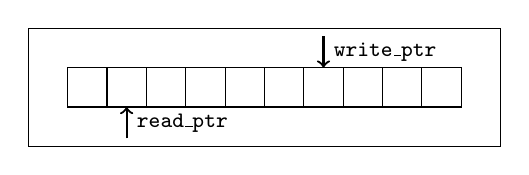
\begin{tikzpicture}
    \path[draw] (0,0) rectangle (6,1.5);
    \foreach \x in {0.5,1,1.5,2,2.5,3,3.5,4,4.5,5}
      \path[draw] (\x,0.5) rectangle (\x+0.5,1);
    \path[draw, ->, thick] (1.25,0.1) -- node [anchor =west] {\footnotesize{\texttt{read\_ptr}}} (1.25,0.5);
    
    \path[draw, ->, thick] (3.75,1.4) -- node [anchor =west] {\footnotesize{\texttt{write\_ptr}}} (3.75,1);      
  \end{tikzpicture}};
  
\node[anchor = north west] at ([xshift=2pt, yshift=-2pt] buf.north west) {Ring buffer};

\path[draw, ->, very thick] (c1.north) |- (buf.west);

\path[draw, ->, very thick] (buf.south-|c2) -- node (mid) {} (c2.north) ;
\path[draw, ->, very thick] (mid.center) -| (c3.north) ;

\path[draw] (-3,-3) rectangle (13,7);
\path[draw, <-, very thick] (c1.south) -- (0,-4) node[anchor = north] {I/O (Sensor)};

\end{tikzpicture}

